\section {はじめに}
鉄道会社Aの特急券予約システムに関する
「特急券予約システムシステムの問題点を推測した仕様」(第\ref{VDMModelExpressReservation}章参照)を、
本来あるべき仕様として書き直した仕様である。

\subsection{本来どうすべきだったのか?}
修正後のクラス図\ref{fig:EvolvedExpressReservationModifiedClassDiagram}で見るように、
本来、特急券予約システムは契約\footnote{口座と言ってもよいが、本モデルでは契約という名前にした}
とリンクが設定されているべきであり、
契約がクレジットカードとリンクしているべきである。

予約会員証も契約を介してクレジットカードを参照できるようにすべきである。

\begin{figure}[h]
	\centering
	{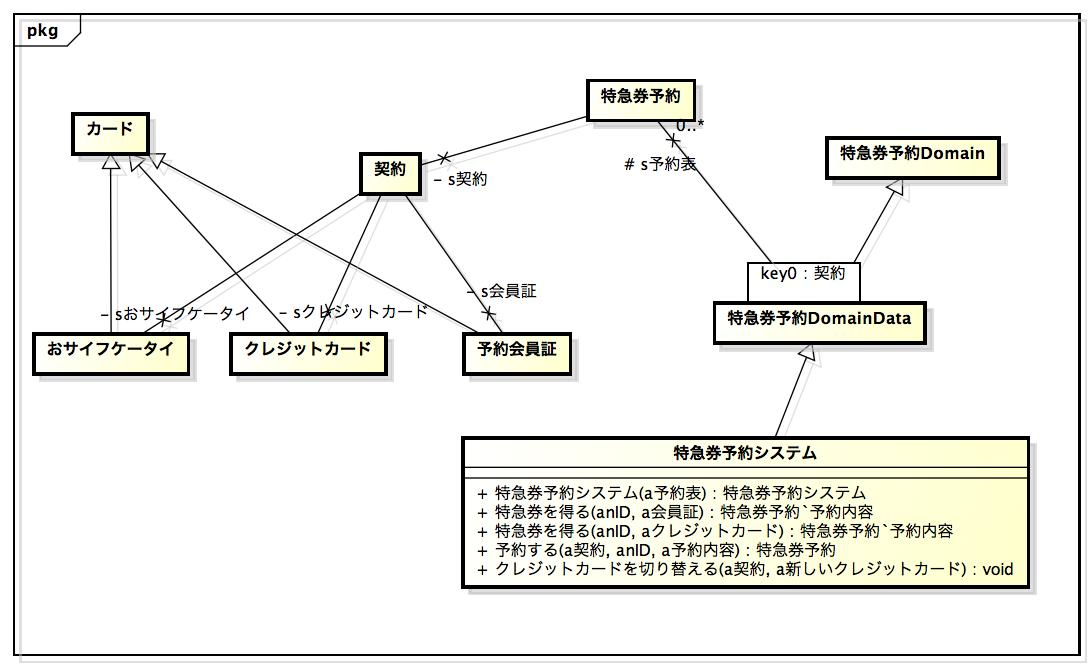
\includegraphics[width=55zw, keepaspectratio]{./EvolvedExpressReservation/image/ModifiedClassDiagram.jpg}}
	\caption{修正後のクラス図}
	\label{fig:EvolvedExpressReservationModifiedClassDiagram}
	\index{しゆせいこのくらすす@修正後のクラス図}
\end{figure}

このようにしておけば、契約に変更があっても、古い特急券予約は新しい契約を介して、新しいクレジットカードにアクセスでき、
同じく予約会員証も新しいクレジットカードにアクセスできる。

修正前のクラス図\ref{fig:ExpressReservationClassDiagram}
と比べれば、再利用性と保守性が増しているにもかかわらず、
構造自体は特に複雑になっているわけではないことが分かる。
